\section{Results}
\label{sec:results}
\subsection{Qualitative Comparison of Encoders}
\label{sec:qualitative}

We begin by comparing encoders qualitatively to build intuition for their behavior before turning to quantitative analyses. 
Representative examples of SCAPE, fixed-scale DoG, Canny, and random control are shown in Figure~\ref{fig:qualitative} (see Section~\ref{sec:experiments}). 
Each method produces distinct patterns in both the encoded stimulus and the resulting phosphene rendering under the default 1024-electrode implant scheme.

Several systematic differences emerge. 
\textbf{SCAPE} emphasizes local contrast while suppressing spurious responses in low-density regions, yielding more interpretable percepts. 
\textbf{Fixed-scale DoG} captures edges but fails to adapt to varying density, leading to oversmoothing in dense regions and excessive detail in sparse ones. 
\textbf{Canny} extracts sharp contours but discards shading, resulting in fragmented and brittle percepts. 
Finally, the \textbf{random control} produces unstructured patterns with no relation to the input, serving as a sanity check. 

These qualitative examples illustrate why adaptive scale selection is important: SCAPE strikes a balance between edge emphasis and clutter suppression that is not achieved by fixed or contour-based baselines. The following sections quantify these observations using representational dissimilarity analysis and reconstruction performance.

\begin{figure}[h!]
    \centering
    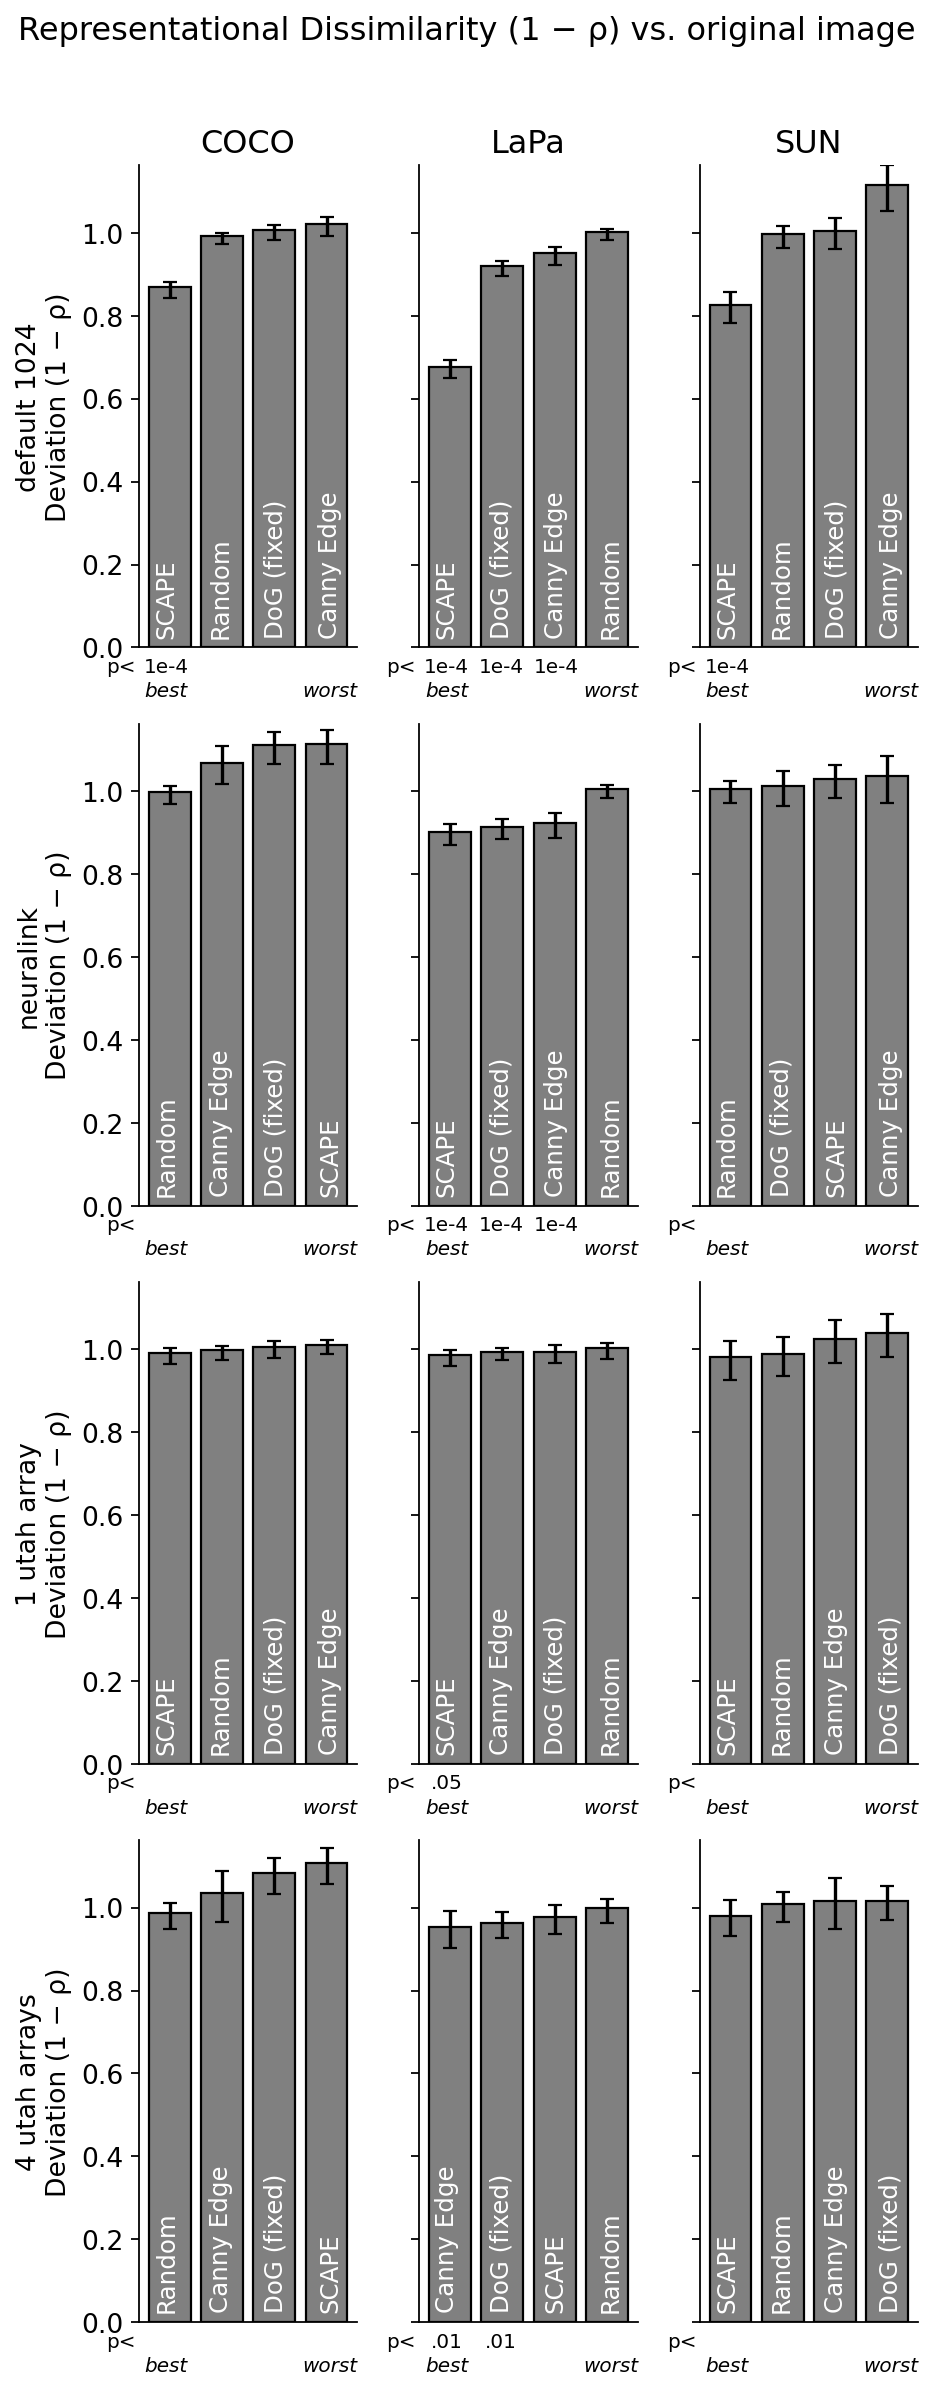
\includegraphics[width=0.9\columnwidth]{figures/RSA.png}
    \caption{\textbf{Representational similarity analysis.} 
    Dissimilarity ($1-\rho$) between phosphene encodings and original image RDMs across COCO, LaPa, and SUN datasets. 
    Bars show mean dissimilarity, error bars denote bootstrap confidence intervals, and $p$-values (permutation test) are reported below each bar. 
    Lower values correspond to greater preservation of structure.}
    \label{fig:rsa_pixel}
\end{figure}


\subsection{Representational Dissimilarity Analysis}
We next assessed the representational fidelity of different phosphene encoding strategies using RSA as defined in Section~\ref{sec:experiments}. 
Figure~\ref{fig:rsa_pixel} shows the dissimilarity of phosphene encodings relative to RDMs across three datasets (COCO, LaPa, SUN) and four implant schemes. 
Lower values correspond to better preservation of the relational structure of the original images.

Across all conditions, \textbf{SCAPE (adaptive DoG)} achieved the lowest dissimilarity, indicating that its density-adaptive filtering preserves similarity structure most effectively. 
The \textbf{fixed-scale DoG} baseline performed moderately well but failed to adapt across sampling densities, leading to higher dissimilarity in sparse layouts. 
\textbf{Canny edges} and the \textbf{random control} consistently produced substantially higher dissimilarities, reflecting poor alignment with stimulus similarity. 
Permutation-based $p$-values (shown below each bar) confirm that SCAPE significantly outperforms the nonadaptive baselines across datasets and implant schemes.


\subsection{Reconstruction Performance}
To complement the representational analysis, we evaluated how effectively a learned decoder could reconstruct natural images from phosphene representations. 
As noted in Section~\ref{sec:experiments}, reconstruction experiments were restricted to the Uniform 1024 scheme. 
Decoder training is specific to each implant layout, and running separate decoders for all schemes would multiply training cost substantially. 
The 1024 layout provides a stable and widely used reference case, making it the most appropriate benchmark for encoder comparison.

Quantitative results are summarized in Tables~\ref{tab:recon_coco}--\ref{tab:recon_sun}, grouped into intensity-based metrics (MSE, SSIM, PSNR) and perceptual similarity metrics (LPIPS, DISTS, MDSI, VSI).
Across all datasets, \textbf{SCAPE} consistently achieved the lowest MSE and the highest PSNR values, indicating superior fidelity in reproducing low-level intensities. 
SSIM scores showed a similar pattern on COCO and SUN, with more modest but consistent gains on LaPa. 
Perceptual metrics confirmed these findings: SCAPE generally outperformed the nonadaptive baselines across datasets, although individual metrics occasionally favored Canny (e.g., MDSI on COCO and SUN). 
Despite such cases, SCAPE provided the best overall balance across metrics, highlighting its robustness to diverse visual statistics.

Qualitative reconstructions further illustrate these trends. 
As shown in Figures~\ref{fig:recon_examples_coco}--\ref{fig:recon_examples_sun}, SCAPE reconstructions preserve continuous shading and object structure, enabling more interpretable outputs. 
By contrast, Canny emphasizes sparse contours at the expense of smooth surfaces, which often fragments object boundaries, while the random control produces severely degraded reconstructions lacking usable structure. 
Taken together, these results demonstrate that adaptive scale selection enables SCAPE to retain substantially more perceptually relevant information than nonadaptive encoding strategies. 
While decoder reconstructions are not direct behavioral measures, the ability to recover more naturalistic scenes suggests that human users may also benefit in perceptual and functional tasks, motivating future behavioral and clinical validation.


\begin{figure}[h]
  \centering
  \includegraphics[width=0.95\columnwidth]{/home/mappel/Dynaphos/spatial_frequency/results/DoG_coco/images/sample_0010.png}
  \includegraphics[width=0.95\columnwidth]{/home/mappel/Dynaphos/spatial_frequency/results/canny_coco/images/sample_0010.png}
  \includegraphics[width=0.95\columnwidth]{/home/mappel/Dynaphos/spatial_frequency/results/random_coco/images/sample_0010.png}
  \caption{Reconstruction examples on COCO under the Uniform 1024 scheme. Each row shows one encoding method: SCAPE (top), Canny edges (middle), and random control (bottom). Columns depict the pipeline from input image to activation map, phosphene rendering, and final reconstruction.}
  \label{fig:recon_examples_coco}
\end{figure}

\begin{figure}[h]
  \centering
  \includegraphics[width=0.95\columnwidth]{/home/mappel/Dynaphos/spatial_frequency/results/DoG_lapa/images/sample_0008.png}
  \includegraphics[width=0.95\columnwidth]{/home/mappel/Dynaphos/spatial_frequency/results/canny_lapa/images/sample_0008.png}
  \includegraphics[width=0.95\columnwidth]{/home/mappel/Dynaphos/spatial_frequency/results/random_lapa/images/sample_0008.png}
  \caption{Reconstruction examples on LaPa faces under the Uniform 1024 scheme. Each row shows one encoding method: SCAPE (top), Canny edges (middle), and random control (bottom). Columns depict the pipeline from input image to activation map, phosphene rendering, and final reconstruction.}
  \label{fig:recon_examples_lapa}
\end{figure}

\begin{figure}[h]
  \centering
  \includegraphics[width=0.95\columnwidth]{/home/mappel/Dynaphos/spatial_frequency/results/DoG_sun/images/sample_0008.png}
  \includegraphics[width=0.95\columnwidth]{/home/mappel/Dynaphos/spatial_frequency/results/canny_sun/images/sample_0008.png}
  \includegraphics[width=0.95\columnwidth]{/home/mappel/Dynaphos/spatial_frequency/results/random_sun/images/sample_0008.png}
  \caption{Reconstruction examples on SUN scenes under the Uniform 1024 scheme. Each row shows one encoding method: SCAPE (top), Canny edges (middle), and random control (bottom). Columns depict the pipeline from input image to activation map, phosphene rendering, and final reconstruction.}
  \label{fig:recon_examples_sun}
\end{figure}




\begin{table}[htbp!]
\centering
\scriptsize
\setlength{\tabcolsep}{2.5pt}   % tighter columns
\renewcommand{\arraystretch}{0.95}
\caption{Reconstruction metrics on the Uniform 1024 scheme across datasets (results restricted to Uniform 1024; see Section~\ref{sec:experiments} for rationale).}

\label{tab:recon_all}

\begin{subtable}{\columnwidth}
\centering
\captionsetup{font=footnotesize}
\caption{COCO}
\label{tab:recon_coco}
\resizebox{\columnwidth}{!}{
\begin{tabular}{lccc cccc}
\toprule
Processing model  & \multicolumn{3}{c}{Intensity reconstruction} & \multicolumn{4}{c}{Perceptual reconstruction} \\
\cmidrule(lr){2-4} \cmidrule(lr){5-8}
  & MSE & SSIM & PSNR & LPIPS & DISTS & MDSI & VSI \\
\midrule
SCAPE & \textbf{0.062} & \textbf{0.592} & \textbf{12.718} & \textbf{0.620} & \textbf{0.424} & 0.559 & \textbf{0.151} \\
Canny & 0.070 & 0.635 & 12.012 & 0.623 & 0.489 & \textbf{0.545} & 0.156 \\
Random & 0.071 & 0.635 & 11.999 & 0.695 & 0.636 & 0.600 & 0.179 \\
\bottomrule
\end{tabular}}
\end{subtable}

\vspace{0.5em}

\begin{subtable}{\columnwidth}
\centering
\captionsetup{font=footnotesize}
\caption{LaPa}
\label{tab:recon_lapa}
\resizebox{\columnwidth}{!}{
\begin{tabular}{lccc cccc}
\toprule
Processing model  & \multicolumn{3}{c}{Intensity reconstruction} & \multicolumn{4}{c}{Perceptual reconstruction} \\
\cmidrule(lr){2-4} \cmidrule(lr){5-8}
  & MSE & SSIM & PSNR & LPIPS & DISTS & MDSI & VSI \\
\midrule
SCAPE & \textbf{0.057} & \textbf{0.500} & \textbf{13.180} & \textbf{0.564} & \textbf{0.382} & \textbf{0.515} & \textbf{0.101} \\
Canny & 0.072 & 0.554 & 12.285 & 0.579 & 0.413 & 0.518 & 0.129 \\
Random & 0.076 & 0.566 & 12.003 & 0.625 & 0.516 & 0.560 & 0.147 \\
\bottomrule
\end{tabular}}
\end{subtable}

\vspace{0.5em}

\begin{subtable}{\columnwidth}
\centering
\captionsetup{font=footnotesize}
\caption{SUN}
\label{tab:recon_sun}
\resizebox{\columnwidth}{!}{
\begin{tabular}{lccc cccc}
\toprule
Processing model  & \multicolumn{3}{c}{Intensity reconstruction} & \multicolumn{4}{c}{Perceptual reconstruction} \\
\cmidrule(lr){2-4} \cmidrule(lr){5-8}
  & MSE & SSIM & PSNR & LPIPS & DISTS & MDSI & VSI \\
\midrule
SCAPE & \textbf{0.054} & \textbf{0.599} & \textbf{13.177} & 0.616 & \textbf{0.433} & 0.563 & \textbf{0.154} \\
Canny & 0.064 & 0.636 & 12.359 & \textbf{0.607} & 0.486 & \textbf{0.548} & 0.156 \\
Random & 0.067 & 0.638 & 12.171 & 0.676 & 0.582 & 0.602 & 0.189 \\
\bottomrule
\end{tabular}}
\end{subtable}
\end{table}